%% %% %% %%
%%
%% Parte B de la práctica
%%
%% %% %% %%

\documentclass[../procedimientos.tex]{subfiles}
\graphicspath{{\subfix{../../images/}}}

\begin{document}
\clearpage
\subsection{Parte B}
\subsubsection{Instrucciones}
\begin{em}
  Programar las funciones expresadas en formato SOP y POS canónicas y mínimas 
  del previo en forma flujo de datos, para su posterior simulación dentro de la plataforma
  \textit{Quartus II}.
\end{em}

\subsubsection{Análisis}\label{subs:analisis_b}
El análisis correspondiente a esta sección se realizó en la sección 
~\ref{subs:previo} ---en la primer pregunta del previo. En ella, se describen 
las funciones deducidas, las cuales se pueden pasar a código. Los mintérminos 
y maxtérminos se encuentras en número, pero el paso a forma algebraica es 
inmediato.

\subsubsection{Implementación en Quartus}\label{subs:b_imp}
Con las formas reducidas anteriormente, se implementó el sistema dentro de la 
plataforma \textit{Quartus II}. Para esto, después de crear un nuevo proyecto, 
se creó un nuevo archivo de tipo \textbf{VHDL}, el cual tiene el contenido 
mostrado a continuación:
\begin{lstlisting}[language=VHDL, caption=Archivo VHDL (Parte B)]
-- Implementacion: Parte B
library ieee;
use ieee.std_logic_1164.all;

entity p04b is
	port(
		a,b,c,d		: in		std_logic;
		f_sop,
		f_pos,
		fr_sop,
		fr_pos 		: out		std_logic_vector(3 downto 0)
	);
end;

architecture simple of p04b is
begin
	-- Forma SOP Simplificada
	fr_sop <= (
		3 => '0',
		2 => a or b or c or d,
		1 => (a and d) or (b and c and d) or (a and b and c)
				or (not a and not b and not c and not d),
		0 => (not a and not b and not c and not d)
				or (not a and not b  and c and d)
				or (not a and b and not c and d)
				or (not a and b and c and not d)
				or (a and not b and c and not d)
				or (a and b and not c and not d)
				or (a and b and c and d)
	);

	-- Forma POS Simplificada
	fr_pos <= (
		3 => '0',
		2 => a or b or c or d,
		1 => (not a or b or d) and (not a or c or d)
				and (a or not b or c) and (a or b or not d)
				and (a or not c or d),
		0 	=> (not a or c or not d)
				and (not a or b or c)
				and (not a or b or not d)
				and (b or c or not d)
				and (a or not b or c or d)
				and (a or not b or not c or not d)
				and (a or b or not c or d)
				and (not a or not b or not c or d)
	);
					
	-- Forma SOP Canonica
	f_sop <= (
		3 => '0',
		2 => (not a and not b and not c and d)
				or (not a and not b and c and not d)
				or (not a and not b and c and d)
				or (not a and b and not c and not d)
				or (not a and b and not c and d)
				or (not a and b and c and not d)
				or (not a and b and c and d)
				or (a and not b and not c and not d)
				or (a and not b and not c and d)
				or (a and not b and c and not d)
				or (a and not b and c and d)
				or (a and b and not c and not d)
				or (a and b and not c and d)
				or (a and b and c and not d)
				or (a and b and c and d),
		1 => (not a and not b and not c and not d)
				or (not a and b and c and d)
				or (a and not b and not c and d)
				or (a and not b and c and d)
				or (a and b and not c and d)
				or (a and b and c and not d)
				or (a and b and c and d),
		0 => (not a and not b and not c and not d)
				or (not a and not b and c and d)
				or (not a and b and not c and d)
				or (not a and b and c and not d)
				or (a and not b and c and not d)
				or (a and b and not c and not d)
				or (a and b and c and d)
	);
	
	-- Forma POS Canonica
	f_pos <= (
		3 => '0',
		2 => a or b or c or d,
		1 => (not a or not b or c or d)
				and (not a or b or not c or d)
				and (not a or b or c or d)
				and (a or not b or not c or d)
				and (a or not b or c or not d)
				and (a or not b or c or d)
				and (a or b or not c or not d)
				and (a or b or not c or d)
				and (a or b or c or not d),
		0 => (not a or not b or not c or d)
				and (not a or not b or c or not d)
				and (not a or b or not c or not d)
				and (not a or b or c or not d)
				and (not a or b or c or d)
				and (a or not b or not c or not d)
				and (a or not b or c or d)
				and (a or b or not c or d)
				and (a or b or c or not d)
	);
end;
\end{lstlisting}

Tal como se puede ver, las salidas del sistema están dada en forma de vector, 
para lo cual se usó el tipo de dato \textit{std\_logic\_vector} y donde $w$ 
era el bit más significativo, mientras que $z$ era el bit menos significativo.  
Tal como se puede ver en el código, se implementaron cuatro funciones 
diferentes:
\begin{itemize}
  \item \textit{fr\_sop}: Forma SOP reducida
  \item \textit{fr\_pos}: Forma POS reducida
  \item \textit{f\_sop}: Forma SOP canónica
  \item \textit{f\_pos}: Forma POS canónica
\end{itemize}

A través de uns simulación funcional en \textit{Quartus II}, se obtuvo el 
siguiente resultado:
\begin{figure}[H]
  \centering
  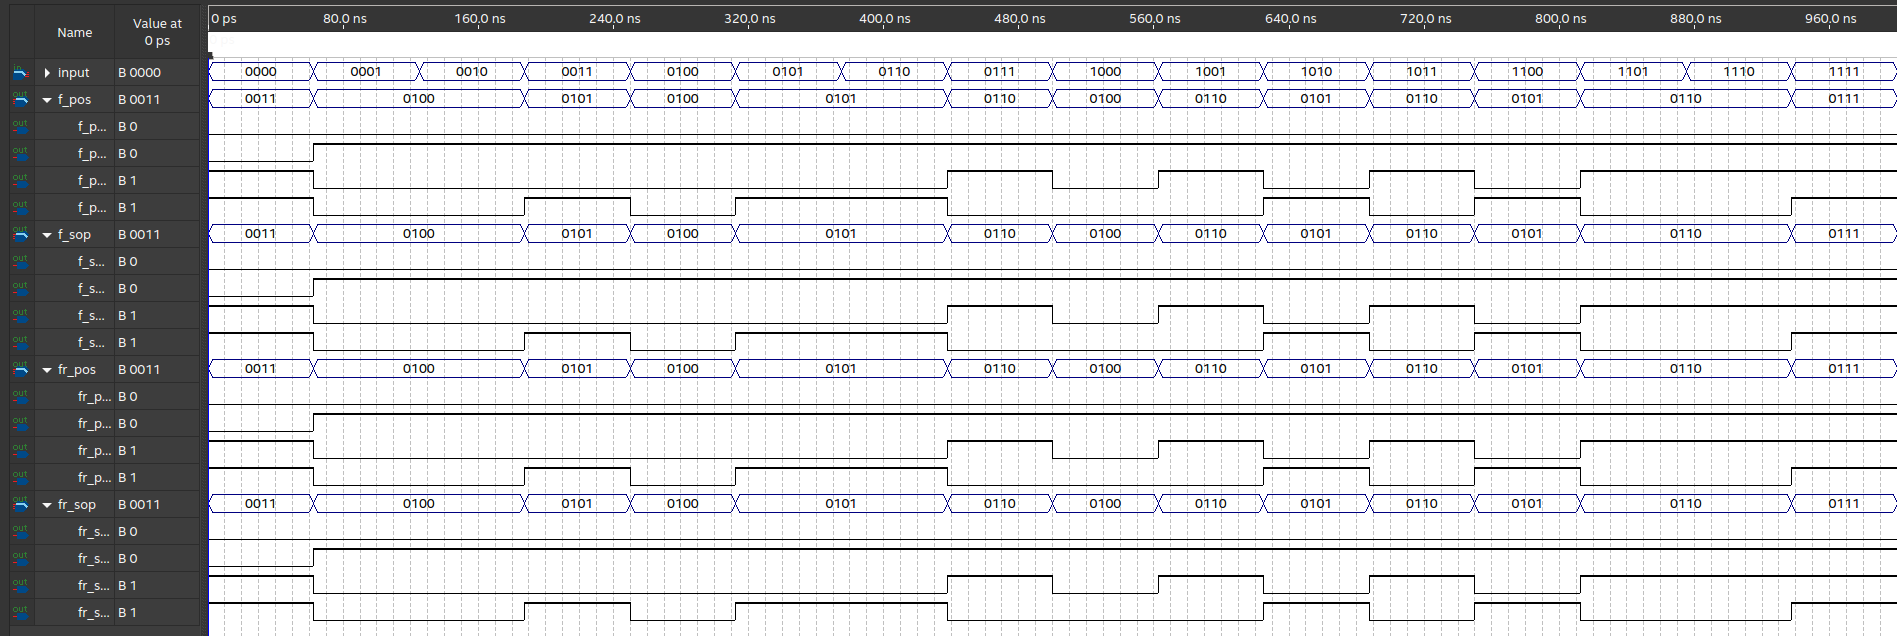
\includegraphics[width=\textwidth]{sim_b}
  \caption{Simulación Funcional (Parte B)}
\end{figure}

El comportamiento del cronograma es el esperado: Tanto la forma SOP canónica; 
la forma POS canónica; la forma SOP reducida; y la forma POS reducida se 
comportan todas iguales.
\end{document}

